\chapter{分离变量法}
\intro{本章详细介绍分离变量法，这是求解有界区域上 PDE 最经典的方法。}

\section{基本思想}

\begin{mydefinition}{分离变量法}
将 PDE 的解表示为各变量独立函数的乘积（或级数），将 PDE 转化为 ODE 求解。
\end{mydefinition}

\section{热传导方程}

\begin{theorem}[分离变量解]
\[
\begin{cases}
u_t=ku_{xx},&0<x<L\\
u(0,t)=u(L,t)=0\\
u(x,0)=\phi(x)
\end{cases}
\]
解为：
\[
u(x,t)=\sum_{n=1}^{\infty}b_n\sin\frac{n\pi x}{L}\exp\left(-\frac{n^2\pi^2kt}{L^2}\right)
\]
其中 $b_n=\displaystyle\frac{2}{L}\int_0^L\phi(x)\sin\frac{n\pi x}{L}\,dx$。
\end{theorem}

\begin{proof}
设 $u(x,t)=X(x)T(t)$，代入方程得 $\frac{T'}{kT}=\frac{X''}{X}=-\lambda$。
分离为两个 ODE：$X''+\lambda X=0$（边值问题）和 $T'+k\lambda T=0$。
特征值 $\lambda_n=(n\pi/L)^2$，特征函数 $X_n=\sin(n\pi x/L)$，叠加即得。
\end{proof}

\begin{figure}[htbp]
\centering
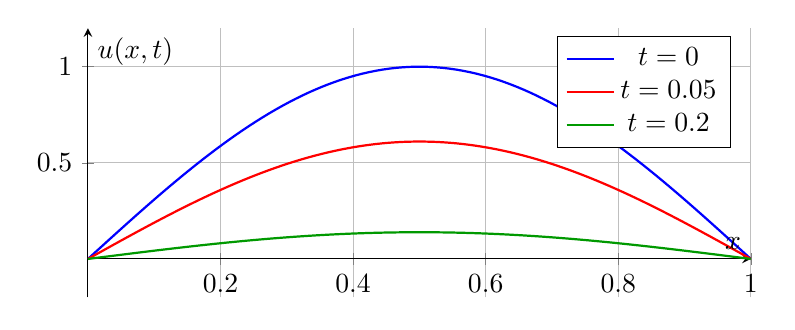
\begin{tikzpicture}
\begin{axis}[
	axis lines=middle,
	xlabel=$x$,
	ylabel={$u(x,t)$},
	xmin=0,xmax=1,
	ymin=-0.2,ymax=1.2,
	legend pos=north east,
	grid=major,
	width=10cm,height=5cm,
]
\addplot[blue,thick,domain=0:1,samples=100]{sin(deg(pi*\x))};
\addplot[red,thick,domain=0:1,samples=100]{sin(deg(pi*\x))*exp(-pi^2*0.05)};
\addplot[green!60!black,thick,domain=0:1,samples=100]{sin(deg(pi*\x))*exp(-pi^2*0.2)};
\legend{$t=0$,$t=0.05$,$t=0.2$}
\end{axis}
\end{tikzpicture}
\caption{分离变量解的演化}
\end{figure}

\section{波动方程}

\begin{theorem}[驻波解]
固定端点弦振动：
\[
u(x,t)=\sum_{n=1}^{\infty}\left(a_n\cos\frac{n\pi at}{L}+b_n\sin\frac{n\pi at}{L}\right)\sin\frac{n\pi x}{L}
\]
每一项对应一个振动模态。
\end{theorem}

\begin{remark}
Neumann 边界条件时，特征函数变为 $\cos(n\pi x/L)$（$n=0,1,2,\ldots$），对应绝热边界。
\end{remark}
